
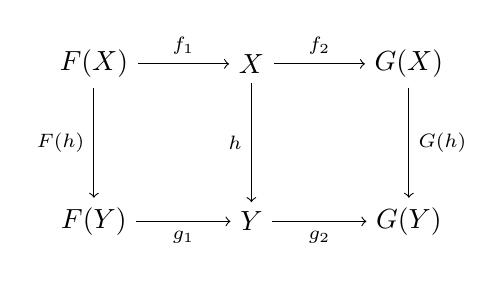
\begin{tikzpicture}[scale=1]
		
	\node (fx) at (0,0) {$F(X)$};
	\node (fy) at (0,-2) {$F(Y)$};
	\node (x) at (2,0) {$X$};
	\node (y) at (2,-2) {$Y$};
	\node (gx) at (4,0) {$G(X)$};
	\node (gy) at (4,-2) {$G(Y)$};
	
	\path[->,font=\scriptsize]
		(fx) edge node[left]{$F(h)$} (fy)
		(x) edge node[left]{$h$} (y)
		(gx) edge node[right]{$G(h)$} (gy)
		(fx) edge node[above]{$f_1$} (x)
		(x) edge node[above]{$f_2$} (gx)
		(fy) edge node[below]{$g_1$} (y)
		(y) edge node[below]{$g_2$} (gy);
			
\end{tikzpicture}

